\chapter{System Design}

\section{Introduction}

The system design phase translates the project requirements into an organized technical blueprint. This chapter outlines the overall system architecture, the 16:9 canvas layout model, Data Flow Diagrams (DFDs), UML diagrams, and the database collection schemas.

\section{System Architecture}

Sentio is built using a clean 3-tier web architecture:
\begin{enumerate}
    \item \textbf{Client Presentation Layer:} Provides specialized web interfaces for Presenters (slide builder and host controls), Projectors (clean 16:9 auditorium display), and Participants (touch-friendly mobile app for voting and answering).
    \item \textbf{Application and Real-Time Gateway Layer:} An Express.js REST API handling user accounts, slide management, and AI requests, combined with a Socket.IO WebSocket server that manages live presentation rooms and instantaneous message broadcasting.
    \item \textbf{Persistence and Services Layer:} A MongoDB database for storing user profiles and presentation decks, along with Groq Cloud AI for fast slide generation and PDFKit for generating session reports.
\end{enumerate}

Figure~\ref{fig:sysarch} illustrates the system architecture and communication paths.

\begin{figure}[H]
    \centering
    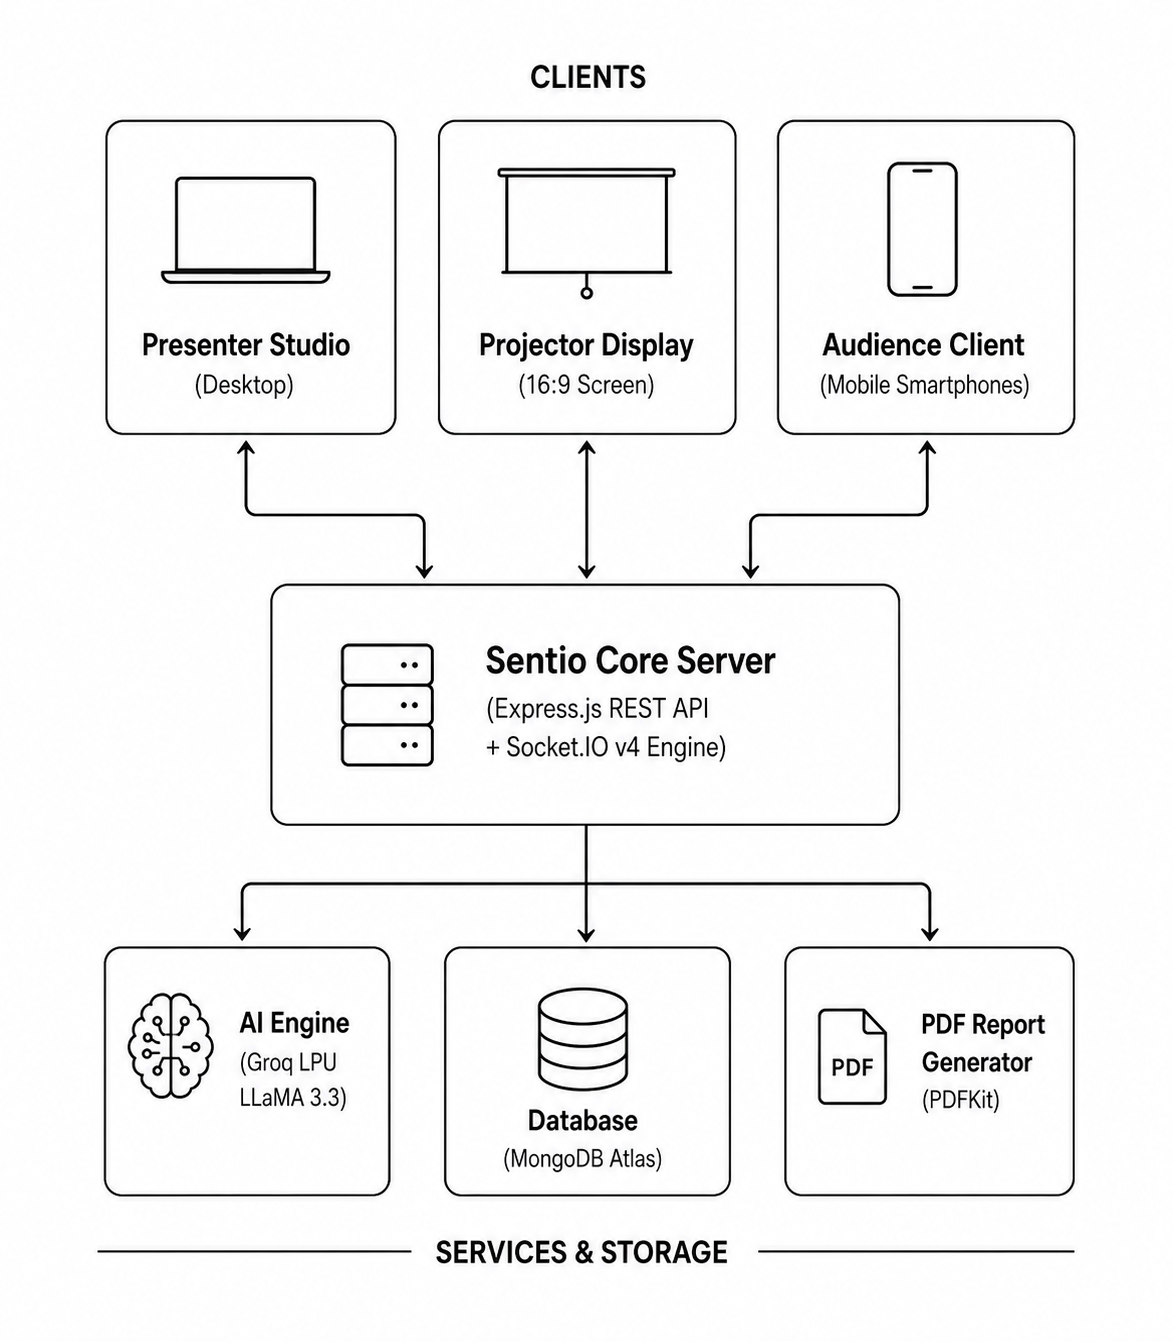
\includegraphics[width=0.9\textwidth]{figures/SentioArchitecture.png}
    \caption{System Architecture of the Sentio Platform}
    \label{fig:sysarch}
\end{figure}

\section{Slide Canvas and Coordinate System}

A fundamental feature of Sentio is the \textbf{Fixed 16:9 Slide Canvas}. In standard web development, text and buttons automatically shift and wrap when the browser window changes size. While this responsive behavior is great for regular websites, it creates problems for presentation slides where titles, images, and questions need to stay in exact visual alignment.

Sentio solves this by using a fixed 16:9 internal coordinate grid ($1920 \times 1080$ units):
\begin{itemize}
    \item Every element placed on a slide—such as headings, body text, pictures, or quiz boxes—has a fixed position and size relative to the slide canvas.
    \item The frontend measures the available screen space and automatically scales the whole slide up or down using CSS transforms while preserving the 16:9 aspect ratio.
    \item This ensures that the slide looks identical whether viewed in the editor, on a laptop, on a large auditorium projector, or on a tablet.
\end{itemize}

\begin{figure}[H]
    \centering
    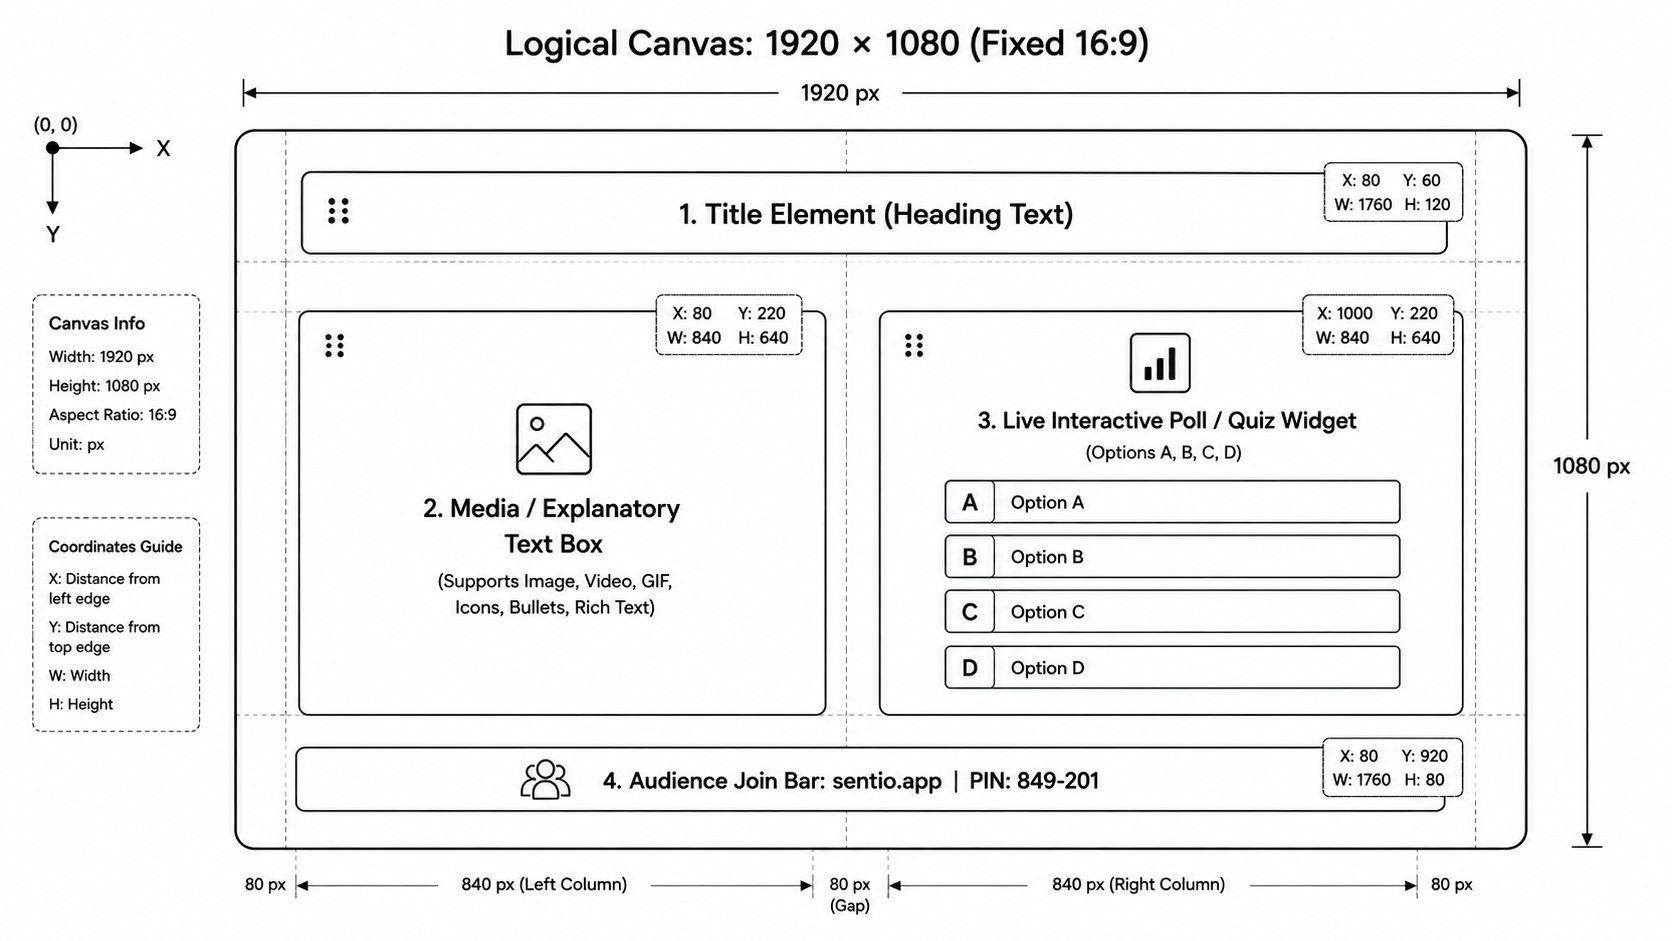
\includegraphics[width=0.85\textwidth]{figures/VisualCanvas.png}
    \caption{Visual Canvas Layout Model}
    \label{fig:canvaslayout}
\end{figure}

\section{Data Flow Diagrams}

\subsection{DFD Level 0 (Context Diagram)}
Figure~\ref{fig:dfd0} shows the high-level data flow between the external actors (Presenter, Participant, and Administrator) and the central Sentio platform.

\begin{figure}[H]
    \centering
    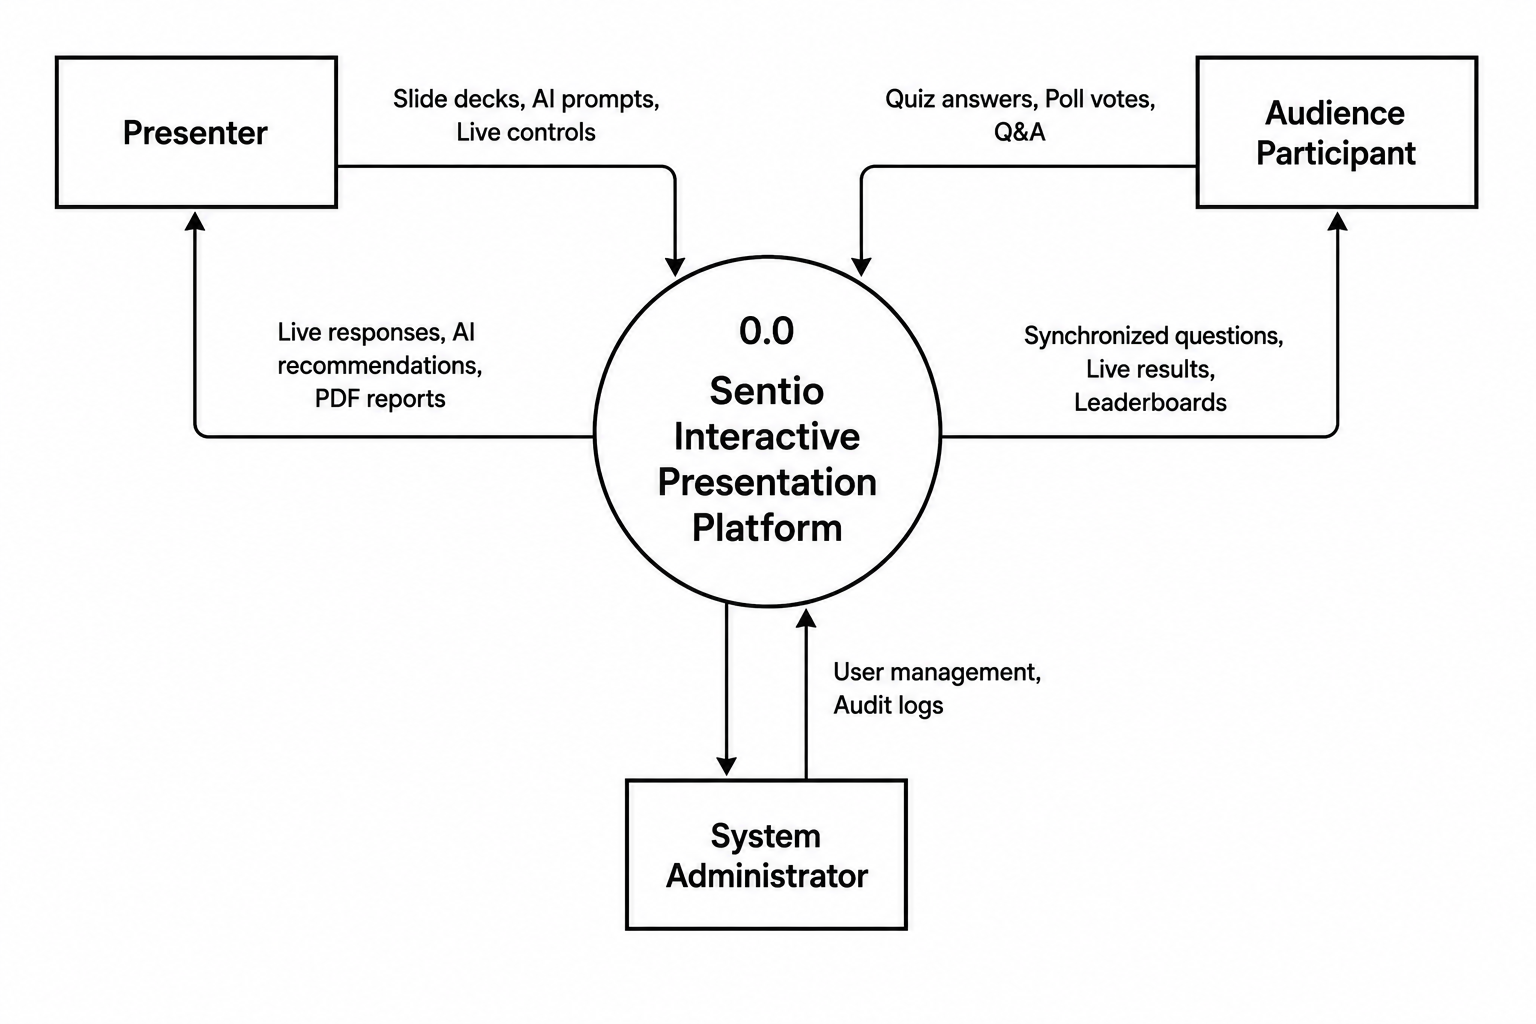
\includegraphics[width=0.85\textwidth]{figures/DFD_Level_0.png}
    \caption{Data Flow Diagram: Level 0 (Context Diagram)}
    \label{fig:dfd0}
\end{figure}

\subsection{DFD Level 1}
Figure~\ref{fig:dfd1} illustrates the internal process breakdown inside the platform, showing how authentication, slide management, AI generation, live session syncing, and reporting interact with the database.

\begin{figure}[H]
    \centering
    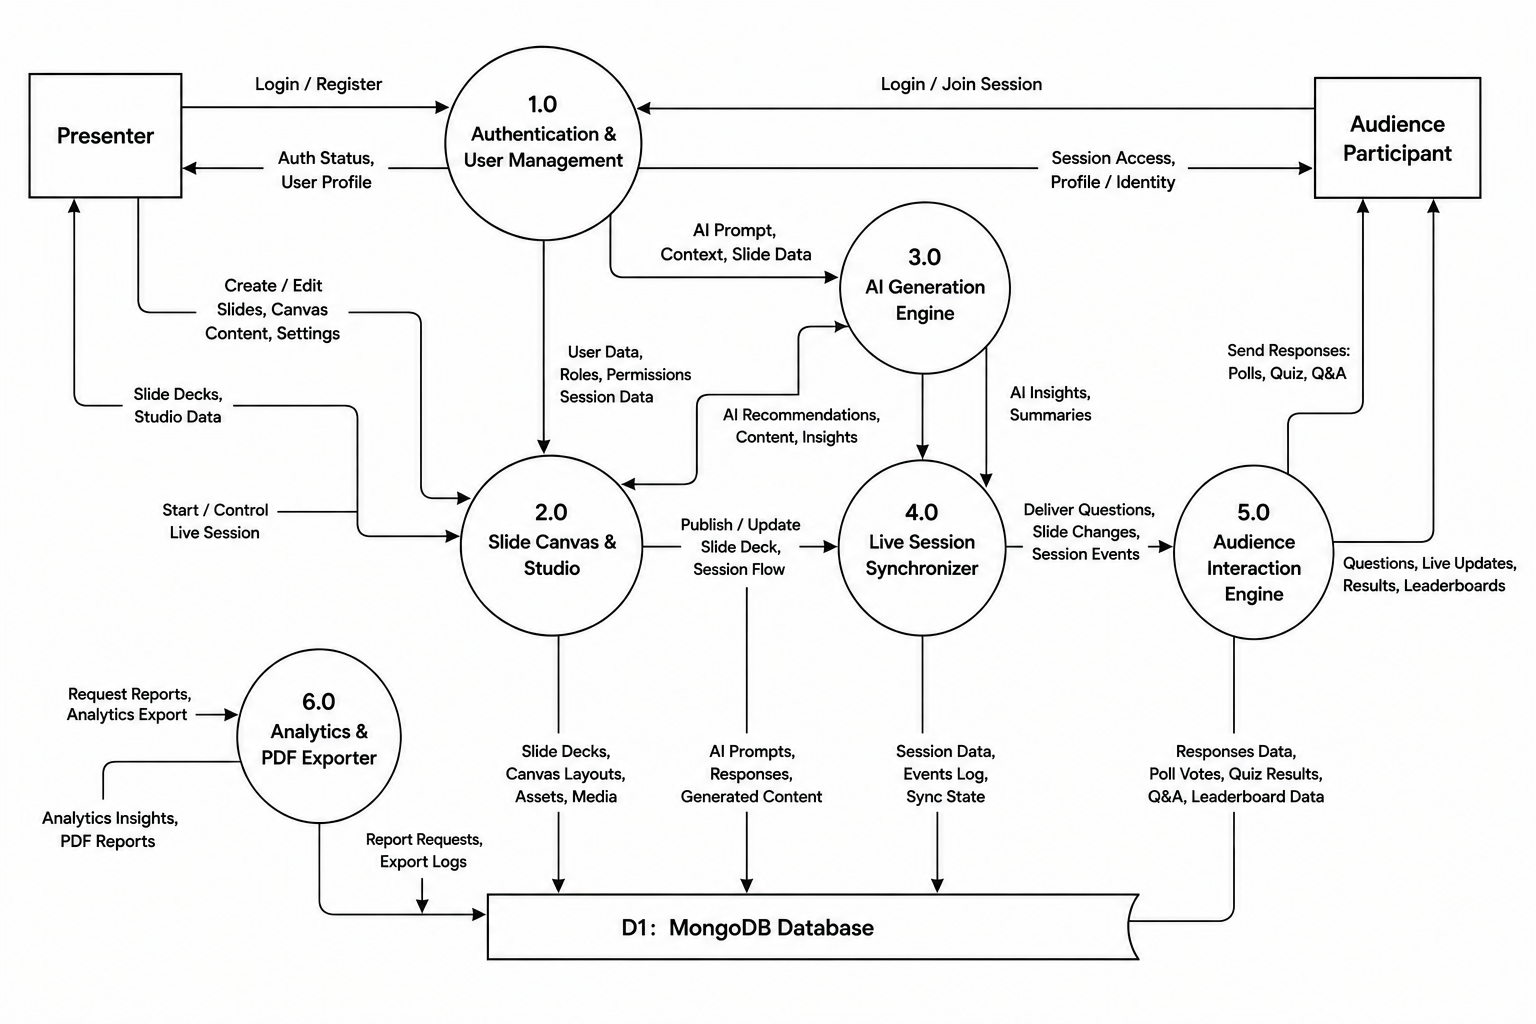
\includegraphics[width=0.9\textwidth]{figures/DFD_Level_1.png}
    \caption{Data Flow Diagram: Level 1}
    \label{fig:dfd1}
\end{figure}

\section{UML Modeling}

\subsection{Use Case Diagram}
Figure~\ref{fig:usecase} illustrates the core functional actions available to Presenters and Audience Participants.

\begin{figure}[H]
    \centering
    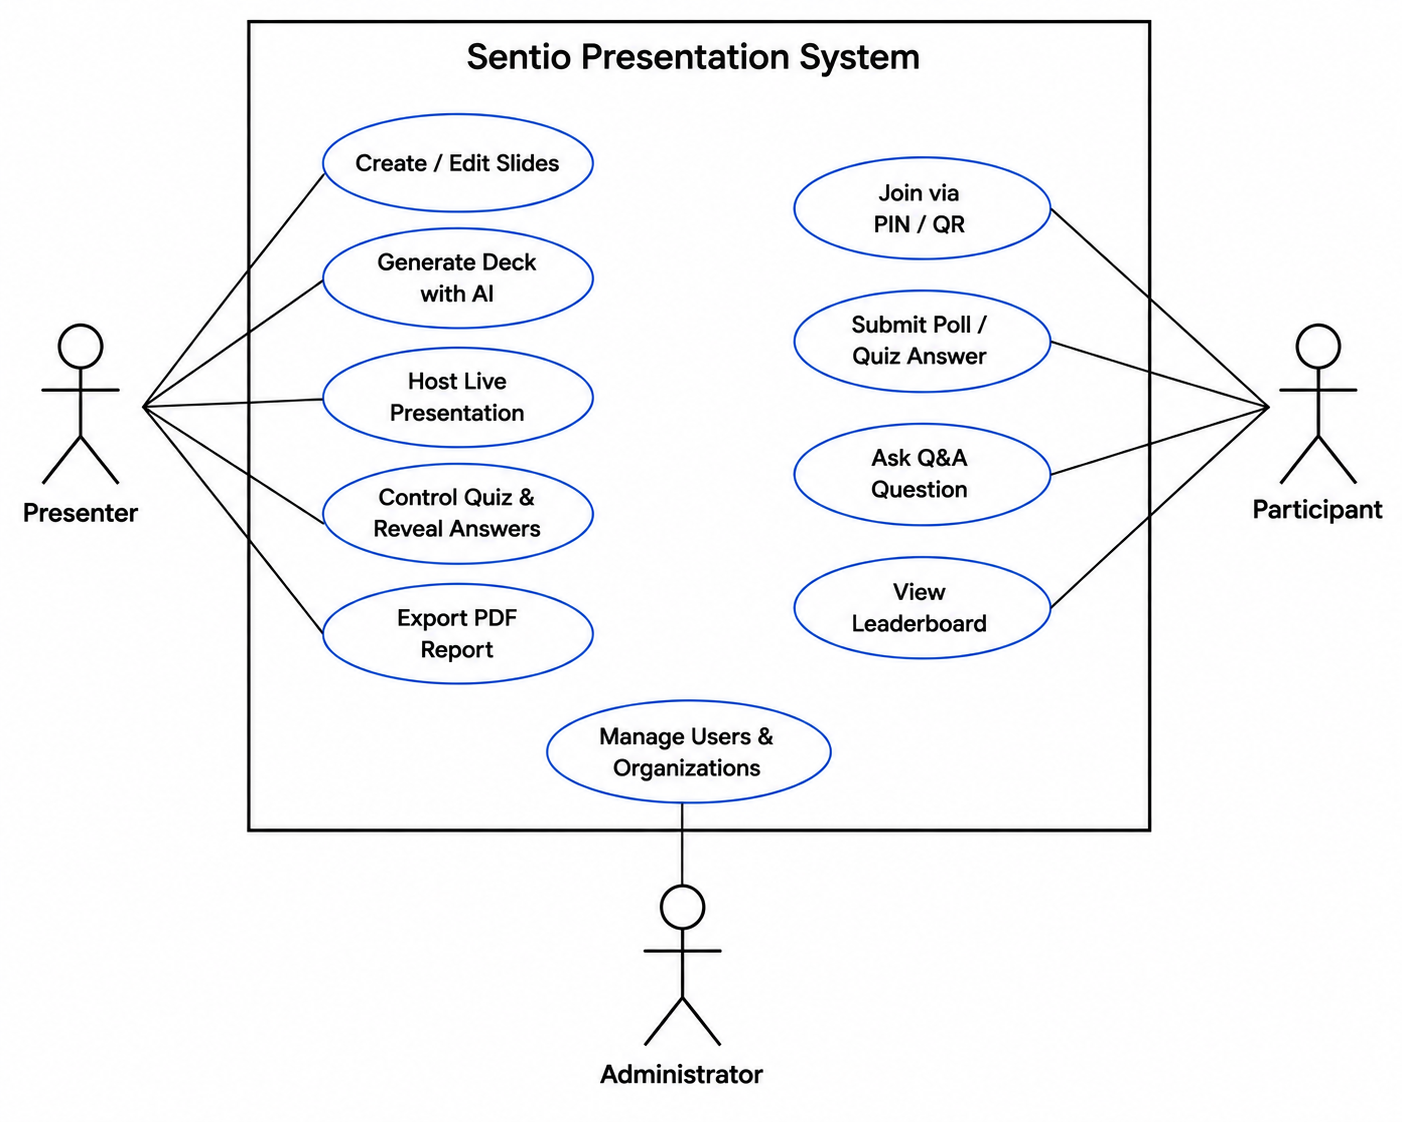
\includegraphics[width=0.85\textwidth]{figures/UML_UseCase.png}
    \caption{UML Use Case Diagram}
    \label{fig:usecase}
\end{figure}

\subsection{Sequence Diagram: Live Interaction}
Figure~\ref{fig:seqdiag} shows the step-by-step sequence of messages exchanged between the presenter, the server, and the audience during a live quiz question.

\begin{figure}[H]
    \centering
    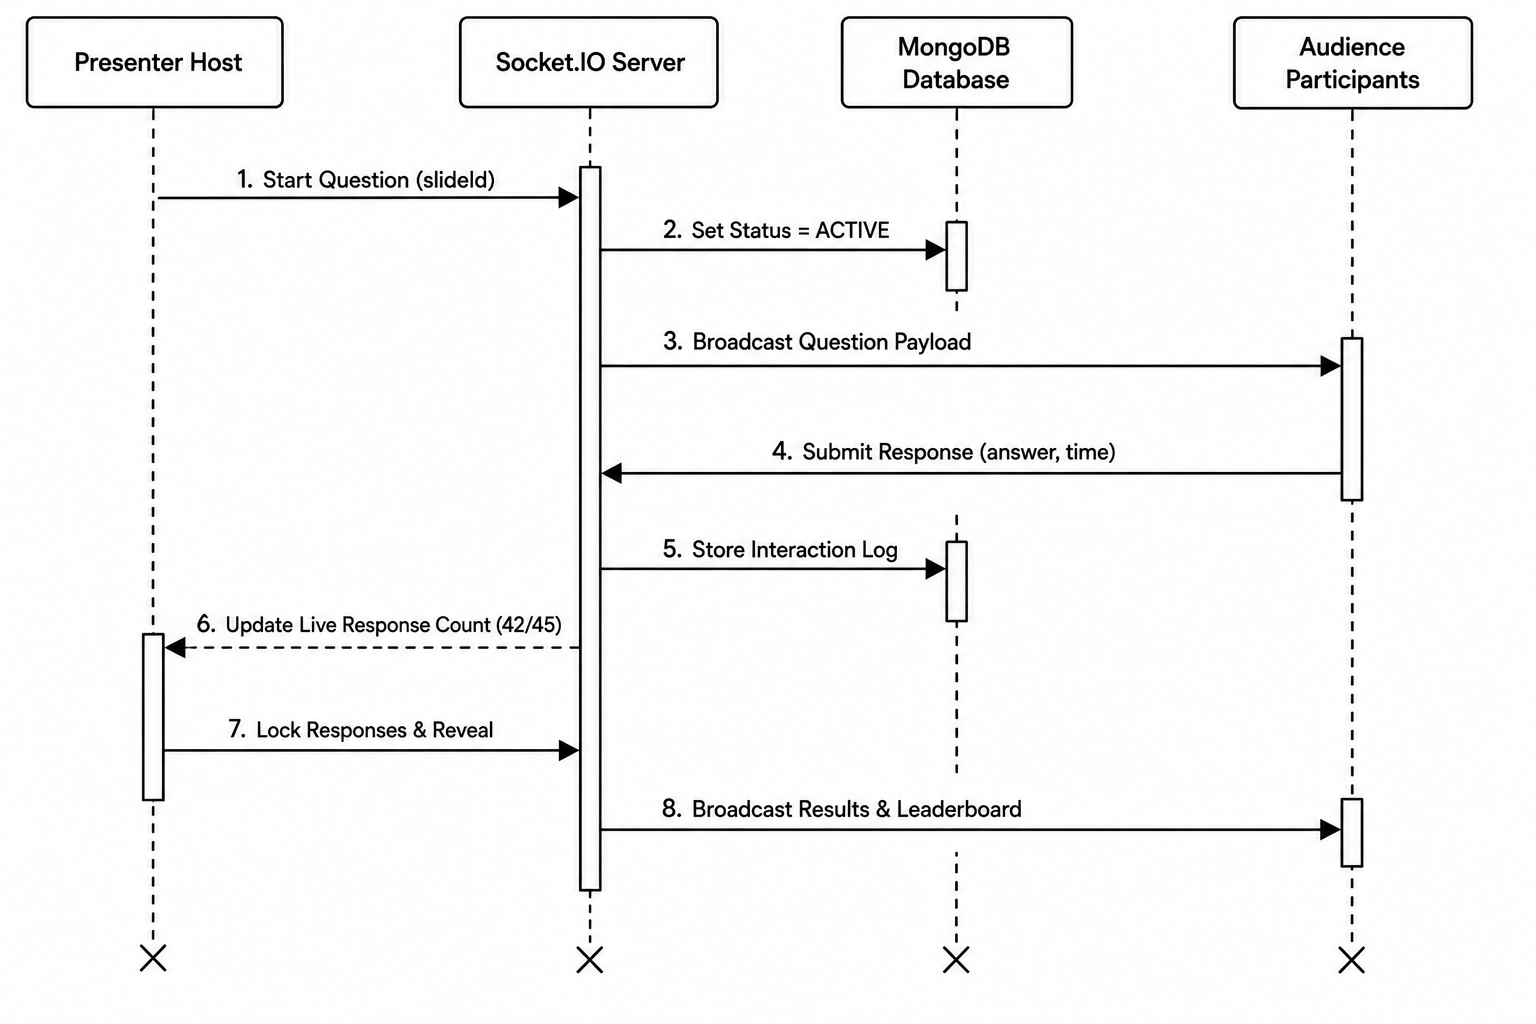
\includegraphics[width=0.85\textwidth]{figures/SequenceDiagram.png}
    \caption{Sequence Diagram for Live Question Flow}
    \label{fig:seqdiag}
\end{figure}

\section{Database Design}

Sentio uses MongoDB to store JSON-based presentation data. The primary collections are described below.

\begin{table}[H]
\centering
\caption{Users Collection (\texttt{users})}
\label{tab:userschema}
\begin{adjustbox}{max width=\textwidth}
\begin{tabular}{llcl}
\toprule
\textbf{Field} & \textbf{Type} & \textbf{Required} & \textbf{Description} \\
\midrule
\texttt{\_id} & ObjectId & Yes & Unique ID for the user \\
\texttt{name} & String & Yes & User's full name \\
\texttt{email} & String & Yes & Unique email address \\
\texttt{passwordHash} & String & Yes & Encrypted password \\
\texttt{role} & String & Yes & Role (\texttt{admin}, \texttt{presenter}, \texttt{participant}) \\
\texttt{createdAt} & Date & Yes & Account creation timestamp \\
\bottomrule
\end{tabular}
\end{adjustbox}
\end{table}

\begin{table}[H]
\centering
\caption{Presentations Collection (\texttt{presentations})}
\label{tab:presschema}
\begin{adjustbox}{max width=\textwidth}
\begin{tabular}{llcl}
\toprule
\textbf{Field} & \textbf{Type} & \textbf{Required} & \textbf{Description} \\
\midrule
\texttt{\_id} & ObjectId & Yes & Unique presentation ID \\
\texttt{title} & String & Yes & Title of the presentation \\
\texttt{creatorId} & ObjectId & Yes & Reference to user \\
\texttt{slidesCount} & Number & Yes & Number of slides in the deck \\
\texttt{createdAt} & Date & Yes & Creation timestamp \\
\bottomrule
\end{tabular}
\end{adjustbox}
\end{table}

\begin{table}[H]
\centering
\caption{Slide Elements Object Structure}
\label{tab:elemschema}
\begin{adjustbox}{max width=\textwidth}
\begin{tabular}{llcl}
\toprule
\textbf{Field} & \textbf{Type} & \textbf{Required} & \textbf{Description} \\
\midrule
\texttt{id} & String & Yes & Unique element ID \\
\texttt{type} & String & Yes & Element type (\texttt{text}, \texttt{image}, \texttt{quiz}, \texttt{poll}) \\
\texttt{x, y} & Number & Yes & Position on 16:9 canvas \\
\texttt{width, height} & Number & Yes & Size on canvas \\
\texttt{properties} & Object & No & Color, font size, and text values \\
\bottomrule
\end{tabular}
\end{adjustbox}
\end{table}